% ----------------------------------------------------------
\chapter{DICIONÁRIO DE PROJETO}\label{cap:desenvolvimento}
% ----------------------------------------------------------
Deve-se inserir texto entre as seções.
% ----------------------------------------------------------
\subsection{Lista de Abreviaturas nos Artefatos do Documento}
Lista de Abreviaturas nos Artefatos do Documento
% ----------------------------------------------------------
\begin{quadro}[htb]
	\centering
	\caption{\label{Formatação do texto.}Requisitos funcionais}	
	\begin{tabular}{|p{4cm}|m{3cm}|p{7cm}|}
		\hline
		\textbf{Artefato} & \textbf{Termo ou sigla} & \textbf{Significado} \\ \hline
		Lista de Requisitos & RF & Requisito funcional: Funcionalidades que um sistema deve possuir. \\ \hline
		Lista de Requisitos & RNF & Requisito não funcional: Características que o software deve possuir, não apresenta funcionalidades. \\ \hline
		Lista de Regras de Negócio & RN & Regra de Negócio: Conjunto de diretizes que orientam como deve ser o funionamente das funcionalidades. \\ \hline
	\end{tabular}
	\fonte{\textcite{Elaborado pelos autores(2023)}.}
\end{quadro}


% ----------------------------------------------------------
\chapter{Referencial teórioco}\label{cap:desenvolvimento}
% ----------------------------------------------------------

% ----------------------------------------------------------
\subsection{React Native}
O React Native é uma poderosa ferramenta de desenvolvimento que permite criar aplicativos móveis nativos para iOS e Android usando JavaScript e a biblioteca React. Essa abordagem eficiente e produtiva para a criação de aplicativos móveis multiplataforma tem impulsionado o crescimento do React Native no mercado.

Desenvolvido e mantido pela empresa META, também proprietária do Facebook, o framework React Native é altamente confiável, beneficiando-se de uma comunidade ativa 
que disponibiliza uma ampla gama de conteúdos gratuitos online. A tendência atual para novos aplicativos móveis é o desenvolvimento voltado principalmente para as 
plataformas Android e iOS. Com o React Native, é possível adotar uma abordagem híbrida, permitindo a construção simultânea de um produto para ambas as plataformas, 
evitando a necessidade de desenvolvimento separado usando as linguagens nativas de cada plataforma, conforme destacado por (\textcite{Sabino}).

Outro fator determinante na escolha do React Native como framework é a sua curva de aprendizado acessível. Devido à ampla familiaridade e popularidade da linguagem 
JavaScript no mundo do desenvolvimento, a adoção do React Native é evidente (Figura 1), destacando sua força e importância no mercado.
\begin{figure}[htb]
	\caption{\label{fig:Fig_1}Linguagem de programção}
	\begin{center}
		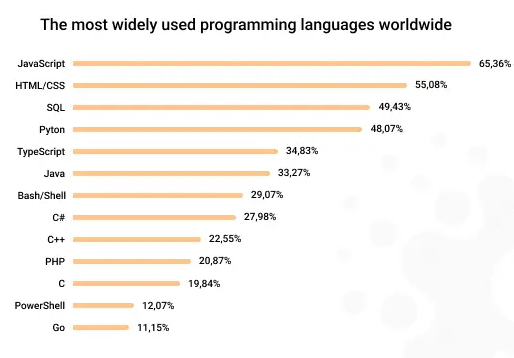
\includegraphics{images/top.png}
	\end{center}
	\fonte{stackoverflow}
\end{figure}
% ----------------------------------------------------------

\subsection{Expo}
O Expo é uma plataforma que simplifica o desenvolvimento de aplicativos móveis usando JavaScript e React Native. Com recursos nativos do dispositivo acessíveis e facilitando a colaboração e distribuição de aplicativos, o Expo oferece uma solução abrangente para criar aplicativos móveis.

Segundo (\textcite{Hugo}) o uso do Expo proporciona uma camada de abstração superior ao React Native, resultando em uma experiência aprimorada no desenvolvimento de software. Com o aumento do 
número de usuários de smartphones, especialmente nas plataformas Android e iOS, a necessidade de criar aplicativos para ambas as plataformas se tornou cada vez mais 
evidente. Nesse contexto, o Expo oferece uma vantagem no desenvolvimento híbrido, simplificando o processo de criação de aplicativos multiplataforma.


\begin{figure}[htb]
	\caption{\label{fig:Fig_1}Expo vantagens}
	\begin{center}
		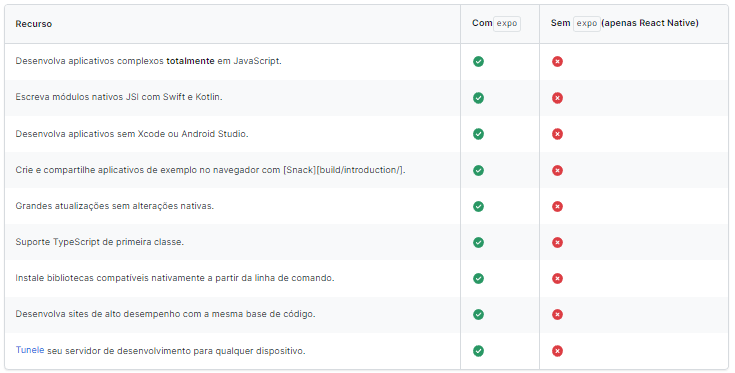
\includegraphics{images/expo.png}
	\end{center}
	\fonte{Expo}
\end{figure}